%!TEX root=paper/thesis.tex
\subsection{Reward definition}\label{sec:det_reward}

The policy's performance at time $t$ is determined by all detections that are part of the set of observations $\mathbf{o}^j$ at the last state $s^j$ before $t$.
Recall that detector actions returns lists of detection hypotheses.
Therefore, the final AP vs. Time evaluation of an episode is a function $eval(h,T_s,T_d)$ of the history of execution $h=s^0,s^1,\dots,s^J$.
It is precisely the normalized area under the AP vs. Time curve between $T_s$ and $T_d$, as determined by the detections in $\mathbf{o}^j$ for all steps $j$ in the episode.

\begin{figure}[h!]
\centering
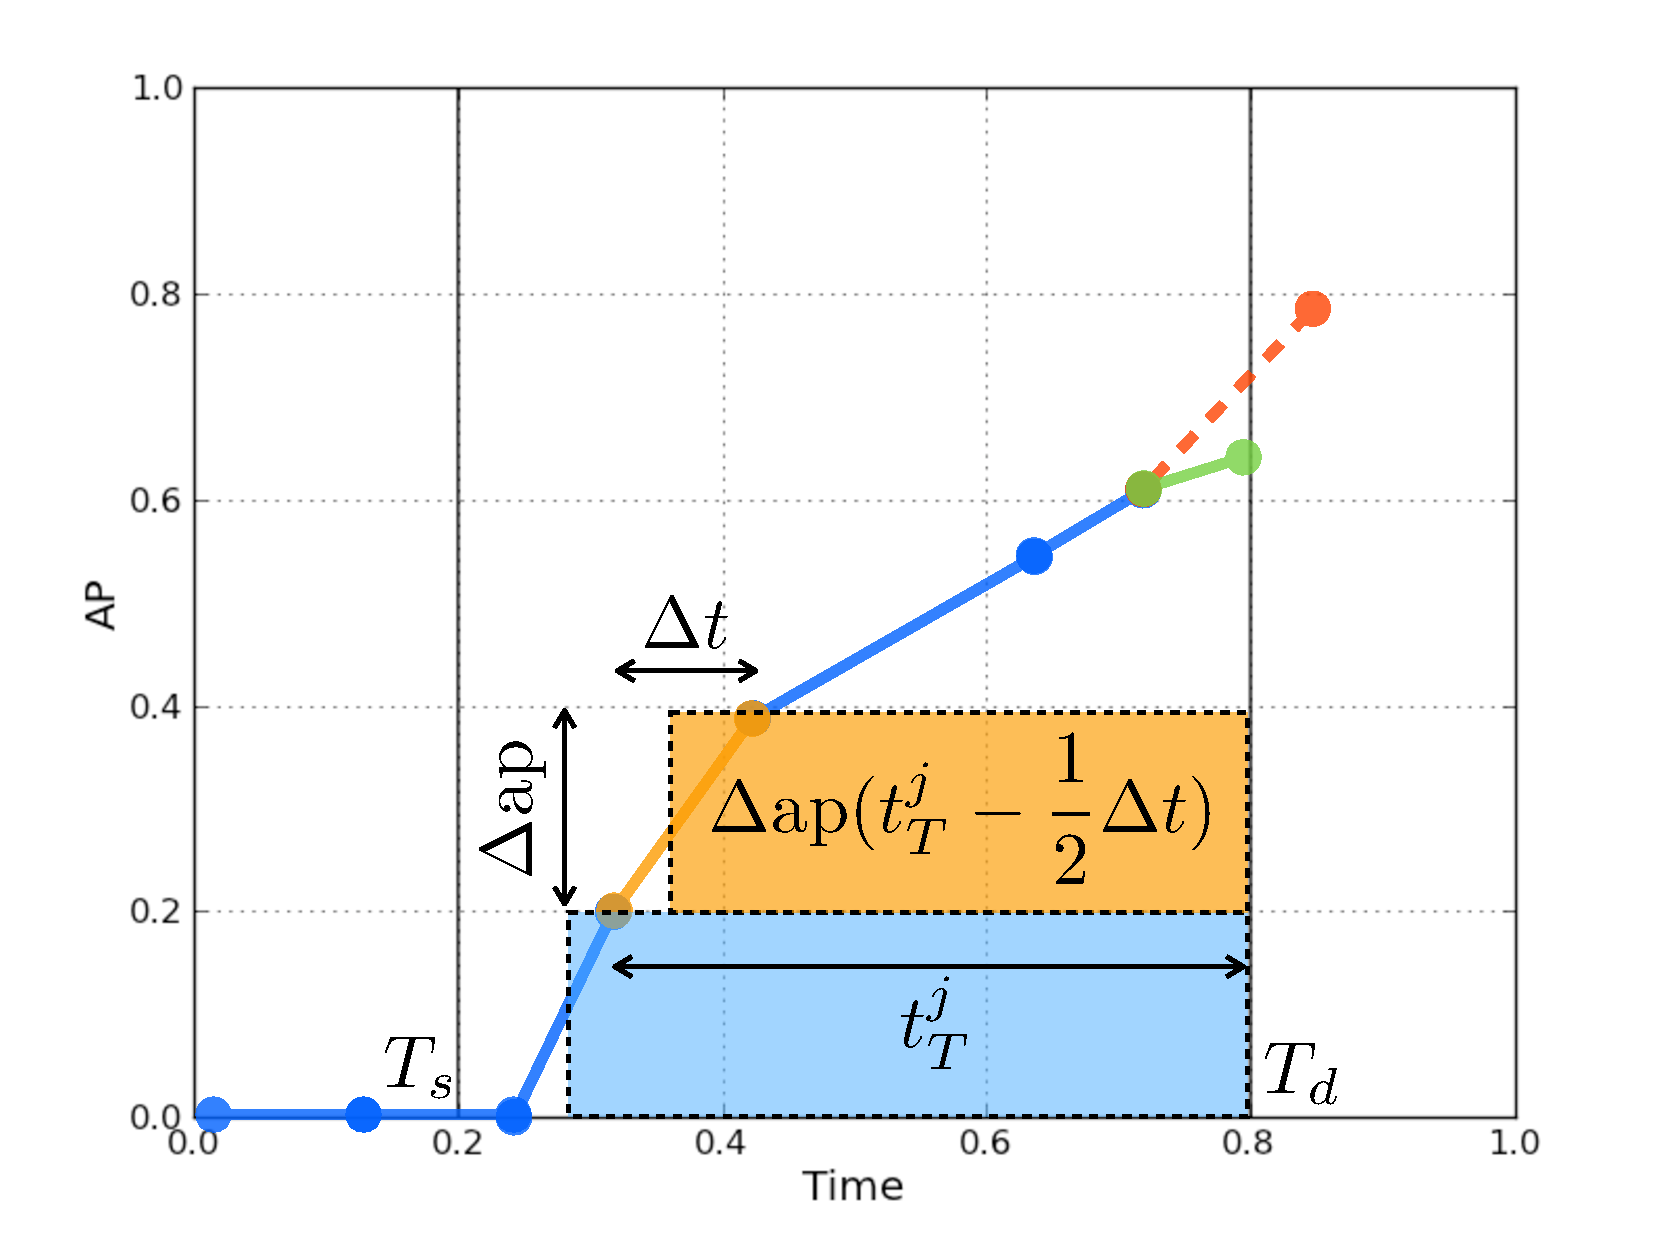
\includegraphics[width=\linewidth]{../../../2011-2012/figures/apvst_expl.pdf}
\caption{
Graphically representing our reward function.
}\label{fig:det_rewards}
\end{figure}


Note from Figure~\ref{fig:det_rewards} that this evaluation function is additive per action, as each action $a$ generates observations that may raise or lower the mean AP of the results so far ($\Delta ap$) and takes a certain time ($\Delta t$).
We can accordingly represent the final evaluation $eval(h,T_s,T_d)$ in terms of individual action rewards: $\sum_{j=0}^J R(s^j,a^j)$.

Specifically, as shown in Figure~\ref{fig:det_rewards}, we define the \emph{reward} of an action $a$ as
\begin{align}\label{eq:advanced}
R(s^j,a) = \Delta \text{ap} (t_T^j-\frac{1}{2}\Delta t)
\end{align}
where $t_T^j$ is the time left until $T_d$ at state $s^j$, and $\Delta t$ and $\Delta \text{ap}$ are the time taken and AP change produced by the action $a$.
(We do not account for $T_s$ here for clarity of exposition.)

\PM{Summary}
In summary, we learn the $\theta$ by \emph{policy iteration}.
First, we gather $(s, a, r, s')$ samples by running episodes (to completion) with the current policy parameters $\theta_i$.
From these samples, $\hat{Q}(s, a)$ values are computed, and $\theta_{i+1}$ are given by $L_2$-regularized least squares solution to $\hat{Q}(s, a) = \theta^T \phi(s, a)$, on all states that we have seen in training.
With pre-computed detections on the PASCAL VOC 2007 dataset, the training procedure takes about $4$ hours on an $8$-core \emph{Xeon E5620} machine.
